\documentclass{article}

% if you need to pass options to natbib, use, e.g.:
% \PassOptionsToPackage{numbers, compress}{natbib}
% before loading nips_2016
%
% to avoid loading the natbib package, add option nonatbib:
\usepackage[nonatbib]{nips_2016}

%\usepackage{nips_2016}

% to compile a camera-ready version, add the [final] option, e.g.:
% \usepackage[final]{nips_2016}

\usepackage[utf8]{inputenc} % allow utf-8 input
\usepackage[T1]{fontenc}    % use 8-bit T1 fonts
%\usepackage{hyperref}       % hyperlinks
\usepackage{url}            % simple URL typesetting
\usepackage{booktabs}       % professional-quality tables
\usepackage{amsfonts}       % blackboard math symbols
\usepackage{nicefrac}       % compact symbols for 1/2, etc.
\usepackage{microtype}      % microtypography
\usepackage{amsmath}
\usepackage{mathtools}
\usepackage{fancyvrb}
\usepackage{multirow}
\usepackage{color}


% HT http://tex.stackexchange.com/a/151987/41154
\DeclarePairedDelimiterX{\infdivx}[2]{(}{)}{%
  #1\;\delimsize\|\;#2%
}
\newcommand{\dkl}{D_\mathrm{KL}\infdivx}

\usepackage{listings}
\definecolor{lightgray}{rgb}{.9,.9,.9}
\definecolor{darkgray}{rgb}{.4,.4,.4}
\definecolor{purple}{rgb}{0.65, 0.12, 0.82}
\definecolor{orange}{rgb}{1,0.5,0}

\definecolor{Red}{RGB}{255,0,0}
\newcommand{\red}[1]{\textcolor{Red}{#1}}
\definecolor{Green}{RGB}{10,200,100}
\definecolor{Blue}{RGB}{10,100,200}
\newcommand{\ndg}[1]{\textcolor{Green}{[ndg: #1]}}
\newcommand{\mht}[1]{\textcolor{Blue}{[mht: #1]}}
\newcommand{\lou}[1]{\textcolor{orange}{[lou: #1]}}

% casual outlining font
\newcommand{\cas}[1]{ \textsf{\color{darkgray} \scriptsize #1} }

\lstdefinelanguage{JavaScript}{
  keywords={typeof, new, true, false, catch, function, return, null, catch, switch, var, if, in, while, do, else, case, break},
  keywordstyle=\color{blue}\bfseries,
  ndkeywords={class, export, boolean, throw, implements, import, this},
  ndkeywordstyle=\color{darkgray}\bfseries,
  identifierstyle=\color{black},
  sensitive=false,
  comment=[l]{//},
  morecomment=[s]{/*}{*/},
  commentstyle=\color{purple}\ttfamily,
  stringstyle=\color{red}\ttfamily,
  morestring=[b]',
  morestring=[b]"
}

\lstset{
   language=JavaScript,
   backgroundcolor=\color{white},
   extendedchars=true,
   basicstyle=\footnotesize\ttfamily,
   showstringspaces=false,
   showspaces=false,
   numbers=none,
   numberstyle=\footnotesize,
   numbersep=9pt,
   tabsize=2,
   breaklines=true,
   showtabs=false,
   captionpos=b
}



\usepackage[ruled,vlined]{algorithm2e}

\newcommand{\ud}{\,\mathrm{d}}
\DeclareMathOperator*{\argmax}{arg\,max}


\title{Practical optimal experiment design for psychology}

% The \author macro works with any number of authors. There are two
% commands used to separate the names and addresses of multiple
% authors: \And and \AND.
%
% Using \And between authors leaves it to LaTeX to determine where to
% break the lines. Using \AND forces a line break at that point. So,
% if LaTeX puts 3 of 4 authors names on the first line, and the last
% on the second line, try using \AND instead of \And before the third
% author name.

\author{
  David S.~Hippocampus\thanks{Use footnote for providing further
    information about author (webpage, alternative
    address)---\emph{not} for acknowledging funding agencies.} \\
  Department of Computer Science\\
  Cranberry-Lemon University\\
  Pittsburgh, PA 15213 \\
  \texttt{hippo@cs.cranberry-lemon.edu} \\
  %% examples of more authors
  %% \And
  %% Coauthor \\
  %% Affiliation \\
  %% Address \\
  %% \texttt{email} \\
  %% \AND
  %% Coauthor \\
  %% Affiliation \\
  %% Address \\
  %% \texttt{email} \\
  %% \And
  %% Coauthor \\
  %% Affiliation \\
  %% Address \\
  %% \texttt{email} \\
  %% \And
  %% Coauthor \\
  %% Affiliation \\
  %% Address \\
  %% \texttt{email} \\
}

\begin{document}
% \nipsfinalcopy is no longer used

\maketitle

\begin{abstract}

Designing good scientific experiments requires ingenuity, rigor, and patience to consider a large space of possible experiments.
With the growing popularity of formal models, part of this time-consuming process can be automated.
Here, we present a general, principled, and turnkey approach to experiment design.
We introduce this framework with the goal to differentiate competing models of psychological phenomena, but the framework is general to any domain where probabilistic models are used.
We implement our system in a user-friendly probabilistic programming language (PPL), allowing for plug-and-play use by the scientist uses PPLs to formalize her hypotheses.
We consider a number of problems specific to psychological phenomena: dealing with noisy responses and deciding on the number of subjects.
We validate our framework using two case studies in the psychology of randomness and categorization.
We find strong empirical validation that our automatically designed optimal experiments were indeed optimal.
Our framework opens up a number of interesting questions, which we explore briefly in the discussion.


\end{abstract}

\mht{I think in practice ``the space of possible experiments'' is the same thing as an ``empirical paradigm''. This terminology may be useful in our exposition.}

\section{Introduction}
\lou{start off more generally, don't specialize too much for psychology.}
Designing scientific experiments is hard.
Scientists must have hypotheses and reason over a potentially large space of possible experiments.
Studying human behavior has additional complications.
Human data is noisy and sensitive to the dependent measure of the task.
Further, human data is expensive and one must balance expected statistical power with the constraints of a limited budget to decide on the number of participants to run.

Formal models of psychological phenomena alleviate some of these issues.
Models make explicit hypotheses about observed data, and thus make it easier (or in some cases, possible) to explore the implications of a set of theoretical ideas.
However, exploring models can be time-consuming and searching through a large space of possible experiments is still largely driven by the scientist's intuition.
This need not be the case: If both the set of hypotheses and the space of experiments are explicit, then we can partially \emph{automate} experiment design as a sort of active learning problem, searching for experiments that maximally update our beliefs about a scientific question.

We present a general, principled, and turnkey approach to designing experiments that uses a Bayesian approach to find experiments that best distinguish competing hypotheses.
The approach is similar in spirit to other Bayesian approaches to experiment design going back to Lindley \cite{Lindley1956} (for a review, see \cite{Chaloner1995}).
We go beyond simple probability models, however, and implement the framework  in a \emph{probabilistic programming language} (PPL), providing new generality to the approach.
PPLs are a convenient and compositional way to represent explicit hypotheses about the data.
We show how optimal experiment design (OED) can be streamlined into a scientist's workflow by instantiating it in a user-friendly PPL in which formal hypotheses can already be expressed.
This is a crucial step in making a practical OED system: Once you're using a PPL to formalize your hypotheses, OED comes for free.
%\lou{as explained, this doesn't seem so crucial to me.}

%Though the framework is Bayesian, it is not directly related to Bayesian models of cognition; rather, it can be applied to any instance in which the scientist has a formal model of the data generating process (including, Bayesian models of cognition).

We are not the first to attempt to develop a framework for optimal experiments in psychology.
Previous attempts (e.g. \cite{Myung2009}), however, suffer from a number of pragmatic issues, including ad-hoc optimization criteria, lack of an established pipeline, and failure to accommodate common worries in psychology experiments (e.g., dealing with noisy responses, determining sample sizes, and selecting dependent measures or linking functions).
% Taken together, these issues put the burden on researchers to have sufficient expertise to adapt the OED system to their specific problem and require researchers to develop their own system for writing formal psychological models and the OED optimization engine.
In this paper, we resolve these issues using a Bayesian model selection framework implemented in a practical modeling system.
We apply this framework to two case studies from cognitive psychology: perceptions of subjective randomness and category learning.
The first case study highlights the details of application for a simple space of experiments.
The second study applies OED to a more realistic space of possible experiments and validates our theoretical analysis by running the optimal experiment.
Our general system opens a number of rich areas for future development, which we explore in the discussion.

%We conclude by highlighting the generality of the approach and areas of future work.
%\ndg{all the parts are here. needs smoothing. make it clearer that using PPL to represent hypotheses is a key step in making the system practical.}

%    \begin{itemize}
%        \item It is difficult to discriminate models of psychological processes
%        \item Experiments are expensive
%        \item We present a general, turn-key approach to design experiments that best disambiguate competing models using a Bayesian framework
%        \item This technique is not directly related to Bayesian models of cognition. It can be used on any (formal / probabilistic) model, including Bayesian models of cognition
%        \item Despite the previous attempts in this field, there are a number of pragmatic issues that make it difficult to readily apply OED techniques for psychology, including:
%        \begin{itemize}
%            \item A variety of proposed optimization criteria, which puts the burden on researchers to have sufficient expertise to select the appropriate approach
%            \item A lack of an established pipeline, requiring researchers to develop a language to formalize psychological models and write an OED optimization engine
%            \item A lack of analysis in dealing with practical experimental concerns such as:
%                \begin{itemize}
%                    \item Noisy responses from participants
%                    \item The ideal number of participants for a study
%                    \item The ambiguity of linking functions of dependent measures
%                \end{itemize}
%        \end{itemize}
%    \end{itemize}


\section{Bayesian model selection framework}
\label{s:bayes}



\cas{because probabilistic programming is so crucial to our work, we give an introduction to the language we use, webppl}

\cas{walk through biased coin, markov coin models}

\cas{re-emphasize 2 benefits of ppls: clear hypotheses, plug and play inference}

\cas{discuss sample(), condition(), factor() (= likelihood weighting), score()}

\lou{we assume that subjects are iid and that each subject's response is conditionally iid given their latent values.. discussion: relax these assumptions, connect with mixed models (maybe having linking functions gives us this?)}

Let $P(X)$ be a prior distribution on experiments, $P(Y)$ a prior on possible responses, and $P(M)$ a prior on models.
A model $m$ is a conditional distribution $P_m(Y \mid X)$ that represents predictions about response data $y_i$ for different possible experiments $x_i$ (we will use the notation $m(x)$ as shorthand for $P_m(Y \mid X = x)$).

The goal of OED is to find the experiment $x^{*}$ that maximizes the expected information gain about the belief distribution on models $P(M \mid X = x^{*})$.
We use KL divergence as our measure of information gain; the optimal experiment $x^*$ maximizes the expected KL divergence over the space of responses:
\begin{align}
x^{*} &= \argmax_{x} \sum\limits_{y} p(y ; x) \dkl{ P(M \mid X = x, Y = y) }{ P(M) } \label{eq:oed}
\end{align}
One natural choice for $p(y ; x)$ is simply an uninformative distribution---this is appropriate if the practitioner does not a priori believe that any models are the true model.
Alternatively, if we do believe that $M$ contains the true model, we could use the predictive distribution implied by the models:
$$ p(y ; x) = \sum\limits_{m}p_m(y \mid x)p(m) $$
where $p_m(y \mid x)$ is the distribution on responses $y$ for experiment $x$ predicted by model $m$.
We discuss the decision criteria for these different response distributions throughout our two case studies.

\subsection{Probabilistic programs}

Complex probabilistic models require new representations to support their specification. Probabilistic programs are such a representation, extending probabilistic graphical models with insights from programming language research.
PPLs provide compositionality and abstraction, which are incredibly useful for articulating clear, formal hypotheses. In addition, PPLs separate model description from implementation, and generic tools for calculating efficient probabilistic inference can be swapped in on a need-to-use basis, depending on the details of the probabilistic model.
We implement our OED system as a probabilistic program, allowing us to harness these features.

We use the probabilistic programming language WebPPL (\url{webppl.org}), a small but feature-rich probabilistic programming language embedded in Javascript \cite{dippl}.
WebPPL uses primitive Distribution objects (e.g. \lstinline{Binomial}), which can be accessed with a number of different methods: \lstinline{sample}, \lstinline{score}, \lstinline{support}.
For instance, \lstinline|sample(Binomial({n: 4, p: 0.5}))| returns a sample from the Binomial distribution with parameters $n=4, p = 0.5$. \lstinline|score(Binomial({n: 4, p: 0.5}), 2)| will return the log-probability of the value 2 under this Binomial distribution.
Oftentimes, we are interested in posterior inference. Let's say we are interested in the Binomial(4, 0.5) distribution conditional on at least 2 positive outcomes. In WebPPL, we would write this as:
%
\begin{lstlisting}[mathescape, label={code:webppl}, caption = {Posterior inference in WebPPL.}]
var myBinomialModel = function(){
	var x = sample(Binomial({n: 4, p: 0.5}))
	condition(x >= 2)
	return x
}
\end{lstlisting}
%
In Listing \ref{code:webppl}, we've constructed a function with no arguments (i.e., a thunk: \lstinline{myBinomialModel}), which samples from a Binomial distribution, uses the WebPPL primitive \lstinline{condition} to specify how we want to update our distribution, and returns the resulting sampled value \lstinline{x}.
\lstinline{condition} looks to see if the condition is satsfied (if $x\geq2$); if it is not, it re-weights the likelihood of that \emph{program execution} (composed of all of the random choices made before the condition statement) to 0.
\lstinline{condition} is a special case of \lstinline{factor}, which adjusts the (log) likelihood of the program execution by some value (most often, the log probability of the data under that program execution).

Notice how this model has not specified \emph{how} we are to construct a posterior distribution. For that, we would call this function with a generic inference routine \lstinline{Infer(myBinomialModel, options)}. In \lstinline{options}, we would specify what inference algorithm we want to use. WebPPL currently has several inference algorithms to choose from: MCMC, full Enumeration, Hamiltonian Monte Carlo, Sequential Monte Carlo, and Variational Inference.

Because we have expressed the space of models, experiments, and responses in the language of probability, it is straightforward to express Equation \ref{eq:oed} as a probabilistic program (see Listing \ref{code:oed-pp}).
This makes it clear that OED is an inference problem.
Attacking this problem using probabilistic programming allows us to separate the task of describing the problem (i.e., writing the generative model of OED) from the task of solving it (i.e., choosing/writing the inference algorithm).
In addition, framing OED this way gives us access to algorithms that are more sophisticated than previous research has considered  (e.g., HMC for continuous experiment spaces).
If we are not interested in the full distribution of information gain, we could substitute in an optimization operator \lstinline{Search()} rather than the posterior inference operator \lstinline{Infer()}.
%\lou{note that outermost Infer() could also be a Search()}

\mht{the \lstinline{infer} used in the code is a little cryptic and doesn't seem to match the way I'm describing \lstinline{Infer()} above}
%\begin{minipage}{\linewidth}
\begin{lstlisting}[mathescape, label={code:oed-pp}, caption = {OED implementation. For clarity, we have omitted some book-keeping details.}]
var OED = function(mSample, xSample, ySample, infer) {
  var mPrior = infer.M1(function() { mSample() })
  infer.X(function() {
    var x = xSample()                       // ${\color{purple} p(x)}$
    var yPredictive = infer.Y1(function() { // ${\color{purple} P(Y = y) = \sum_{m} p_m(y \mid x)p(m) }$
      var y = ySample(), m = sample(mPrior)
      factor(score(m(x), y))
      return y
    })
    var KLDist = infer.Y2(function() {  // ${\color{purple} \sum_{y} p(y) \dkl{ P(M \mid Y = y) }{ P(M) } }$
      var y = sample(yPredictive)
      var mPosterior = infer.M2(function() {
        var m = sample(mPrior)
        factor(score(m(x), y))
        return m.name
      })
      return KL(mPosterior, mPrior)
    })
    var EIG = expectation(KLDist)
    factor(EIG)
    return {x: x, EIG: EIG}
  })
}
\end{lstlisting}
%\end{minipage}
Our OED code is available as a WebPPL package---see \url{https://github.com/mhtess/webppl-oed}.

\section{Case study 1: Subjective randomness}
\label{s:tutorial}

We demonstrate our OED system in an intuitive and restricted domain: subjective randomness.
Human judgments about randomness are surprisingly systematic and nonuniform across equally likely outcomes -- for example, a sequence of outcomes of coin flips \lstinline{HTHTTTHH} is considered to be more random than the sequence \lstinline{HHHHHHHH} ~\cite{goodfellow38:jep, griffiths01:cogsci}.
%This discrepancy between human intuitions and statistical fact about randomness has garnered significant attention from both the mathematical~\cite{chaitin01:er, kac83:as, li97:kca} and psychological~\cite{falk81:pme, lopes82:jep, griffiths01:cogsci} literature.

There are many hypotheses one might have about what underlies human intuitions about randomness.
Here, we consider three simple hypotheses in the domain of coin flipping: (a) \emph{Weighted coin}: participants reason about the weight of the coin (i.e., the probability of a \lstinline{H} outcome), (b) \emph{Markov coin}: participants reason about the transition probabilities between \lstinline{H} and \lstinline{T} outcomes, and (c) \emph{Fair coin}: participants assume coins flipped are fair coins.
We consider an experimental setup where participants observe four flips of the same coin and are asked to predict the outcome of the next flip.


\subsection{Model space}


Formally, the set of models is $\{m_{\text{weighted}}, m_{\text{markov}}, m_{\text{fair}}\}$, the set of experimental designs $\mathcal{X}$ is the set of all possible sequences of four coin flips, and the set of responses $\mathcal{Y}$ is a choice between heads or tails for the fifth flip.

\lou{add fair coin + 3-model power analysis?}\\
\mht{add number of subjects analysis?}

\subsubsection{Weighted coin model}
\label{s:tutorial:sss:biased}

The weighted coin model models a participant who assumes that coin that generated the observed sequence has some unknown bias and that each coin flip is independent.\footnote{This is a model of a \emph{person's model} of the situation. For more details on this kind of cognitive modeling, see \url{https://probmods.org}}
In this model, the weight of the coin is inferred from the observed sequence of flips by trying to generate the observed sequence, and conditioning on the generated sequence matching the observed sequence.
The inferred coin weight is subsequently used to predict the next coin flip. We show the model in Listing~\ref{lst:m_weighted}.

\begin{lstlisting}[caption=Biased coin model,  label={lst:m_weighted}]
var coinWeights = [0.01,0.1,0.2,0.3,0.4,0.5,0.6,0.7,0.8,0.9,0.99]

var weightedCoin = function(seq) {
  Enumerate(function(){
    var biasProb= uniformDraw(coinWeights);
    var flipWeightedCoin = function(){return flip(biasProb)};
    var sampledSequence = repeat(seq.length, flipWeightedCoin);
    condition(arrayEquals(seq,sampledSequence));
    return flipWeightedCoin()
  })
}
\end{lstlisting}

%
The model first samples a coin weight \lstinline{biasProb} from a discretized uniform distribution over coin weights, and
then makes a helper function \lstinline{flipWeightedCoin} which will flip the weighted coin.
The model then generates a sequence of coin flips of the length of the sequence observed \lstinline{repeat(seq.length, flipWeightedCoin)} and conditions on this matching the observed sequence \lstinline{seq}.
The built-in function \lstinline{condition} rejects executions of the program that fail to match the condition \lstinline{arrayEquals(seq,sampledSequence)}.
The model returns the outcome of the next coin flip.
The model specification is called with an inference algorithm (here, \lstinline{Enumerate} --- which fully enumerates the entire probability distribution), and returns the posterior distribution on the model's return value (here, the outcome of the next coin flip).
%posterior predictive distribution over the next outcome \lstinline{flip(bias_p)}.

\subsubsection{Markov coin model}
\label{s:tutorial:sss:markov}
The Markov coin model assumes that the coin is generated by a Markov process where each coin flip depends on the previous coin flip. The probability of transitioning from the current coin flip is inferred from the experiment prompt sequence, and is subsequently used to predict the next coin flip.

\begin{lstlisting}[caption=Markov coin model]
var markovCoin = function(seq) {
  Enumerate(function(){
    var switchProb =  uniformDraw(coin_weights);
    var sampleOne = function(lastFlip) { flip(switchProb) ? !lastFlip : lastFlip }
 	  var sampleSequence = function(flipsSoFar, n) {
      var nextFlip = sampleOne(last(flipsSoFar))
      return (n == 0) ? flipsSoFar
                      : sampleSequence(append(flipsSoFar, nextFlip),
                      		n - 1) };
	  var sampledSequence = sampleSequence([flip(0.5)], seq.length - 1)
    condition(arrayEquals(seq, sampledSequence));
    return sampleOne(last(sampledSequence))
  })
}
\end{lstlisting}

This model samples a transition probability \lstinline{switchProb} from a discretized uniform distribution over probabilities.
We create a helper function \lstinline{sampleOne}, which returns the opposite of the last outcome with probability \lstinline{switchProb}.
We then generated a sequence of flips according this transition probability beginning with a randomly initialized sequence, using the recursive function \lstinline{sampledSequence}.

\subsubsection{Fair coin model}
\label{s:tutorial:sss:fair}

Our final model assumes participants judgments of randomness are verdical according to flipping a fair coin. In WebPPL, the model looks like:

\begin{lstlisting}[caption=Fair coin model,  label={lst:m_fair}]
var fairCoin = function() {
  Enumerate(function(){
    return flip(0.5)
  })
}
\end{lstlisting}

\subsection{Predictions of optimal experiment design}

We run OED by calling the \lstinline{OED} function on a distribution of models and a distribution of experiments; it then returns the expected information gain for every experiment (Fig.~\ref{fig:run-coin}).
We first explore the expected information gain of experiments designed to disambiguate the fair coin model from the weighted coin model (Figure \ref{fig:run-coin}, left).
We see that the most informative experimenters here are \lstinline{HHHH} and \lstinline{TTTT}.
This makes intuitive sense --- the weighted model would infer a strongly biased coin and make a strong prediction, while the fair coin model is unaffected by the observed sequence.

\begin{figure}[h]
\underline{\textsf{Input:}}
\begin{lstlisting}
OED({mSample: function() { uniformDraw([fairCoin, weightedCoin]) }),
     xSample: function() { repeat(4, flip) }, // experiment space
     ySample: function() { flip() }) // response space
\end{lstlisting}

\underline{\textsf{Output:}}\\
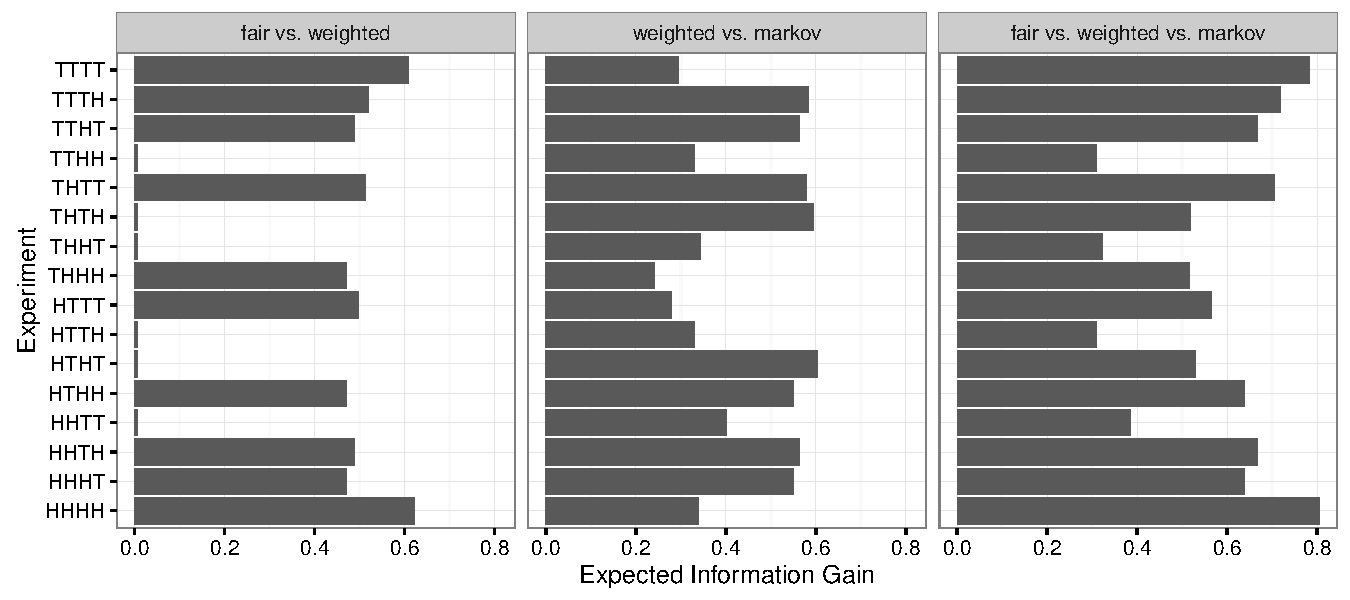
\includegraphics[width=\columnwidth]{img/coin_eig.pdf}
\caption{Running OED in the subjective randomness domain \mht{this is with the number of subjects that we collected; might want to make this for n = 1 (or n = 20) to highlight the symmetries}} \mht{Note this is also with the ignorance prior}
%\lou{make this figure in ggplot, clean it up}
\label{fig:run-coin}
\end{figure}

We also explore the experiments designed to disambiguate the weighted coin model from the Markov coin model (Figure \ref{fig:run-coin}, middle).
We see that \lstinline{HTHT} and \lstinline{THTH} are the most informative experiments, here.
This is also fairly intuitive -- the weighted model infers a 0.5 probability of heads and so assigns equal probability of heads and tails to the next flip, whereas the Markov infers that the probability of transitioning from one outcome to the other is quite high and assigns high probability to the opposite of the last observed value (\lstinline{T} for \lstinline{THTH} and \lstinline{H} for \lstinline{HTHT}).
We also see that \lstinline{HHHH} and \lstinline{TTTT} are now the least informative experiments.
Informally, this is because the models make the same predictions for these experiments, albeit for different reasons.
For instance, for \lstinline{HHHH}, the weighted model infers a high probability of heads and so assigns high probability of heads to the next flip.
The Markov model infers a low probability of transitioning from heads to tails, so it also assigns a high probability of heads to the next flip.

%Finally, the expected information gain of experiments designed to disambiguate all three models is more complex to understand.
%The information gain now depends on how well the experiments disambiguate all three models. Here, we see that for


\subsection{Empirical validation of optimal experiment design}
We validated our OED system by running all of the experiments in the experimental space and comparing the expected information gain with the empirically measured information gain.

\subsubsection{Experimental procedure}

We recruited 320 participants from Amazon's Mechanical Turk. The procedure consisted of a single experiment from the experimental space (i.e. a sequence of 4 coin flips). Participants were randomly assigned to an experiment and generated each coin flip by pressing a button, until all outcomes were shown. Participants then made a prediction about the outcome of the next coin flip (either heads or tails). All of the 16 possible experiments were completed by 20 unique participants. The experiment took about 30 seconds and participants were compensated \$0.10 for their involvement. The experiment in full can be viewed at \url{http://stanford.edu/~mtessler/oed/oed/experiments/subjective-randomness/experiment.html}

\subsubsection{Results}

For each experiment $x_i$ and result $y_i$, we compute the expected information gain from running 20 participants\footnote{because we do client-side randomization, N's are not actually 20; we use the empirical N's for EIG} and compare this to the actual information gain,
$$\mathrm{AIG} = \dkl{P(M \mid Y = y_i, X = x_i)}{P(M)}$$
for different model comparison scenarios.
Figure \ref{fig:aig_vs_eig} shows that expected information gain is a reliable predictor of the empirical value of an experiment (minimum $r$ = 0.857).

\begin{figure}[h!]
\centering
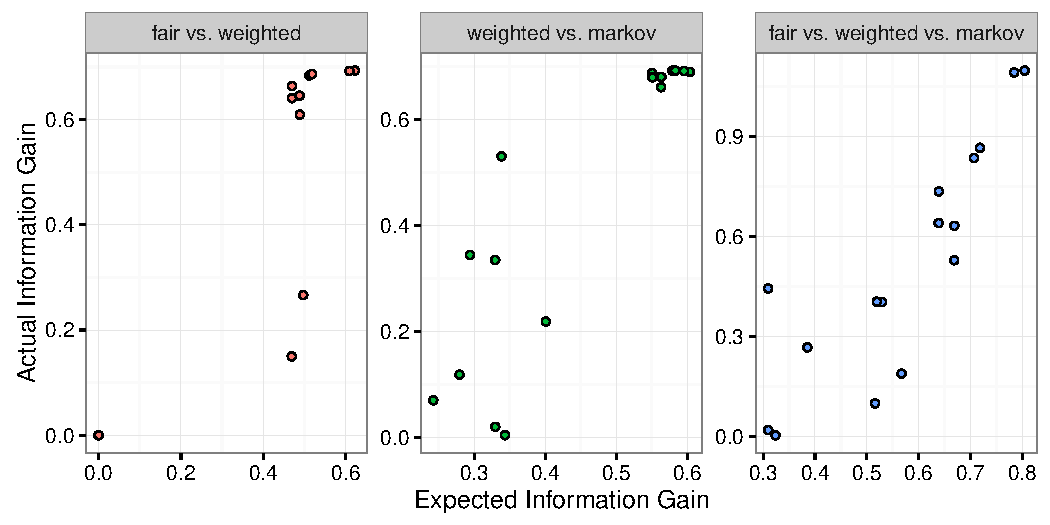
\includegraphics[width=0.7\columnwidth]{img/coin_eig_aig_scatter_noText.pdf}
\caption{Actual information gain vs. Expected information gain for three model comparison setups.}
\label{fig:aig_vs_eig}
\end{figure}

\section{Case study 2: Category learning}

Optimal experiment design has the possibility of addressing experiment and model spaces of arbitrary complexity. Our second case study explores how OED addresses a more realistic space of models and experiments.

We analyze a classic paper in the psychology of categorization aimed to distinguish two competing models of category learning -- the \emph{exemplar model} and the \emph{prototype model} \cite{medin78:pr}. What is particularly interesting about this example is that Medin and Schaffer, the original authors, cleverly designed their experiment with the goal of disambiguating formal models.
From an information-theoretic perspective, how good was the experiment that Medin and Schaffer designed?
Using OED, we find that there are many superior experiments that Medin and Schaffer could have designed but did not.\footnote{Our work here is an exercise in counterfactual history; the exemplar and prototype models, as expressed in the Medin and Schaffer work, are not state of the art models. We chose the Medin and Schaffer research (rather than newer work) as an object of study because it commits to a clear set of competing models and a clear and tractable set of possible experiments.}

In this case study, the models are more complex than the subjective randomness models, which make it difficult to think through the predictions of each.
Further, the experimental space is substantially larger than the subjective randomness experiment space. In the subjective randomness experiment, there were 16 unique experiments. Here, we consider a space of 933 unique experiments.


%
%Medin and Schaffer found that the exemplar model better fit the results of this experiment, and determined it the better model of human category learning.
%
%\lou{rewrite this paragraph}
%%We now consider a richer example in the domain of category learning.
%
%The ability to form concepts and abstract rules establishes a foundation for naming objects and events and is an integral component to cognition.
%Classifying observations and experience into categories is a fundamental learning phenomenon, and models of classification learning have been an active area of research in cognitive science for decades~\cite{machery10:bbs}.
%


%\lou{worth noting that having oed allows us to determine information-theoretic value of the MS experiment.}

% and illustrates how automated experiment design can outperform human intuition. In particular, this case study demonstrates the efficacy of OED in psychology for discrete and non-ordinal experiment spaces, large combinatoric experiment spaces, and parametric model classes.

\subsection{Models}

Both exemplar and prototypes models can be viewed as classifiers that map inputs (here, a vector of boolean features) to a probability distribution on the outputs (a category label: A or B).
The exemplar model assumes people store information about every instance of the category they have observed; categorizing an object is thus a function of the object's similarity to all of the examples of category A versus the similarity to all of B's examples.

By contrast, the prototype model assumes assumes that people store a measure of central tendency for each category---a prototype.
Categorization of an object is thus a function of its similarity to A prototype  A versus its similarity to the B prototype.\footnote{The original prototype model of Medin and Schaffer gave ordinal predictions; we consider a transformation of this model that gives continuous predictions.}

Formally, the exemplar model classifies an object $s$ as an A with probability:
$$ f_e(s ; w) = \frac{ \sum\limits_{r \in A}{\sum\limits_{i}\max (w_i, \delta_{s_i, r_i})} }{
  \sum\limits_{r \in A}{\sum\limits_{i}\max (w_i, \delta_{s_i, r_i} )} + \sum\limits_{r \in B}{\sum\limits_{i}\max (w_i, \delta_{s_i, r_i})}} $$
where $w$ is a free parameter of dimensional weights.

The prototype model classifies an object $s$ as an A with probability:
$$ f_p(s ; w, \alpha, \beta) = \mathrm{logit}^{-1}\left\{ \alpha \times \left[ \beta |R \cap \{s\}| + \sum\limits_{i}w_i \left(2\frac{|\{r \in R ; r_i = s_i \} \cap A |}{|\{r \in R ; r_i = s_i \}|} - 1\right) \right] \right\}$$
where $w$ is a vector of weights, $\alpha$ is an extremizing parameter, and $\beta$ is a bias parameter for objects that have been encountered before.
For details, see the supplementary materials.

\subsection{Experiments}

In the experiments, human participants learn about the category structures in an initial training phase, performing supervised learning of a subset of the objects, and then are tested on this learning in a test phase.
In the training phase, participants see a subset of the objects presented one at a time and must label each object.
Initially, participants can only guess at the labels but they receive feedback so that they can eventually learn the category assignments.
After reaching a learning criterion, they complete the test phase, where they label all the objects (training set and the held out test set) without feedback.

Medin and Schaffer (MS) used visual stimuli that varied on 4 binary dimensions (color: \emph{red} vs. \emph{green}, shape: \emph{triangle} vs. \emph{circle}, size: \emph{small} vs. \emph{large}, and count: \emph{1} vs. \emph{2}).
For technical reasons, they considered only experiments (1) having linearly separable decision boundaries and (2) containing 5 A's and 4 B's in the training set.
There are, up to permutation, 933 experiments that satisfy these constraints.
This space is roughly two orders of magnitude larger than the space of subjective randomness experiments we considered before, although it is small enough to fully enumerate in a reasonable amount of time.

%\cas{4 binary dimensions - 16 objects total}

%\cas{constraints: 9 training stimuli (5 A's and 4 B's)}

%\cas{measure: recall and transfer}

\subsection{Results of optimal experimental design}

We found that the best experiment had an expected information gain of 0.08 nats (for one participant), whereas the MS experiment had an expected information gain of only 0.03 nats; thus, the optimal experiment is expected to be 2.5 times more informative than the MS experiment.
Indeed, the MS experiment only the \red{N}th best experiment (Figure~\ref{fig:dist}a)

\begin{figure}[h!]
\centering
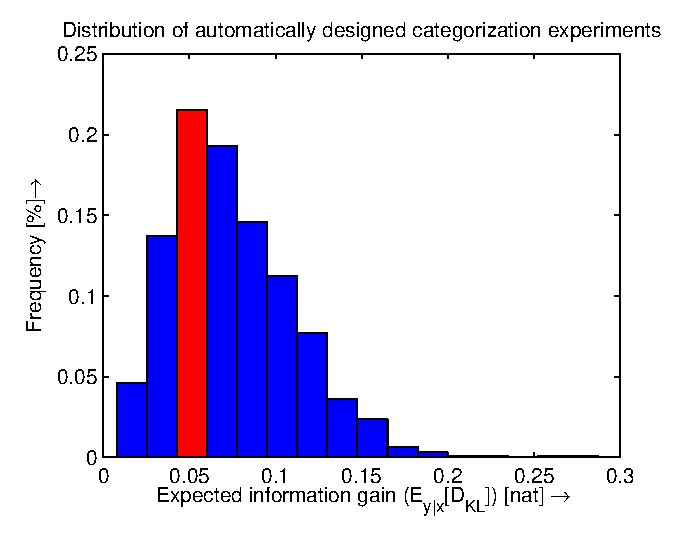
\includegraphics[width=2.5in]{img/dist.eps} 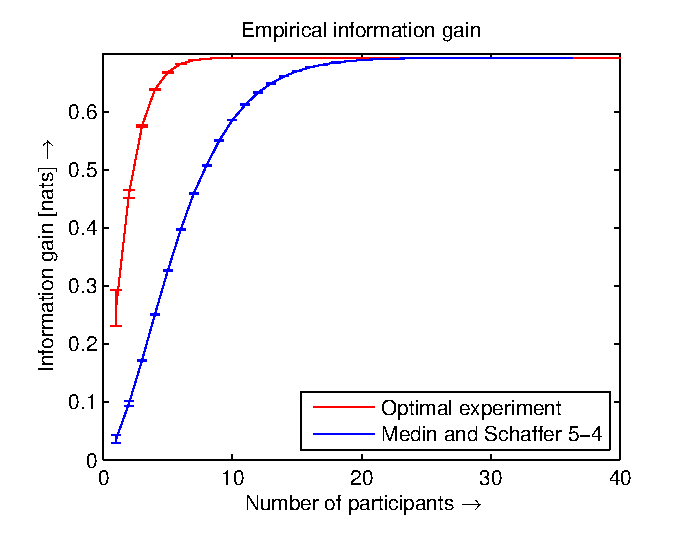
\includegraphics[width=2.5in]{img/empirical.eps}
\caption{Comparing MS experiment with optimal experiment. MS experiment has lower expected information gain and requires twice as many participants to achieve maximum actual information gain.}
\label{fig:dist}
\end{figure}

To validate this finding, we ran both experiments with 40 participants.
Figure~\ref{fig:dist}b shows that, while both experiments give maximal actual information gain with 40 participants, the optimal experiment reaches this maximum with only 8 participants, whereas the MS experiment requires 20.

\subsection{Discussion}

The MS uses a qualitative swap in ranking for two stimuli to disambiguate the models.
However, this prediction has a relatively small magnitude and comes at the expense of little information gain from the remaining stimuli.
The optimal experiment is better able to quantitatively disambiguate the models by maximizing the information from all the stimuli simultaneously
\lou{note that the OED framework is quite flexible. in our model space, we can also encode hard constraints like ``the models must predict different rank orderings''}


\cas{explain different scales for theoretical versus empirical information gain}

\section{Related work}

%\lou{myung \& pitt -- good but requires manually deriving equations for every new experiment design setup}


We are not the first to attempt optimal experiment design for psychology.
Most recently, Myung \& Pitt have introduced a Design Optimization procedure for disambiguating models \cite{Myung2009}.
While a good first step, their procedure unfortunately requires the scientist to specify the optimization criterion for each unique case. For instance, they use the Fisher Information Approximation for disambiguating retention models because these models have similar numbers of parameters but take different functional forms. Other optimization criteria might be appropriate if the models were different. They admit ``the specific choice among such measures would be dependent upon the goals and preference of the experimenter, its computational feasibility, and interpretability considerations.''
We see the need to specify the optimization criteria separately for each case study as a prohibitive burden for the scientist and a roadblock towards widespread adoption.

The problem we address is similar in spirit to problems in active learning.
\lou{Near-Optimal Bayesian Active Learning with Noisy Observations + whocites}
\lou{find related active learning stuff}


\section{General discussion}

%\lou{related work on value of information? (e.g., emma pierson's cogsci paper)}
%
%\lou{look into wikipedia article on bayesian experimental design}



Scientists aim to design experiments that maximize the informativeness of the results.
Our approach partially automates this process, using probabilistic programming in the service of a kind of active Bayesian model comparison.
With our framework, the scientist need only articulate her hypotheses in probabilisitic programs, a convenient and compositional formal framework, and have an idea of the space of possible experiments within an empirical paradigm.
Empirical paradigms are no strangers to the scientific method and are arguably where the genius of experimental work is to be found.
Formal hypotheses have been steadily gaining popularity, and the inclusion of an automated method for experiment design will only accelerate this adoption.

Another roadblock overcome with our framework is the usability of the system.
We implement our approach is a user-friendly probabilisitic programming language which also has the expressive capacity to instantiate modern probabilisitic models.
This means that a framework for probabilisitic modeling can automatically take advantage of optimal experiment design, with no further development needed on behalf of the scientist.
In addition to usability, the fact that our OED is posed as an inference problem in a probabilistic program enables the adoption of new inference strategies as they become available.
For example, if the experimental paradigm describes a continuous space of possible experiments (e.g. if stimuli vary along a continuous dimension like color), inference strategies like Hamiltonian Monte Carlo or Variational Inference, both of which are currently available in WebPPL, might prove useful.


Automatic experiment design
\cas{our work does not replace scientists -- it still requires human intelligence to make models, design an experiment space, and set up measures. instead, it frees them to work on more interesting stuff}

\lou{could easily use something other than KL, e.g, TV distance}

\lou{future research: inference techniques specialized for this domain (e.g., you don't need to estimate $m_1(x)$ and $m_2(x)$ perfectly if you have evidence that $m_1(x) \approx m_2(x)$)}

\lou{make connections to AB/multivariate testing}

\lou{say some stuff about OED for non-psych experiments (e.g., physics)}

\lou{extending to parameter-free predictions?}

\lou{could prove particularly useful in studies of patient populations (difficult/impossible to get high N, so you really wanna make sure the experiment counts)}

\bibliographystyle{ieeetr}
\bibliography{oed_nips_2016}

\end{document}
